\chapter{Le calorimètre SDHCAL}
\label{chap:sdhcal}

\section{Motivation du concept SDHCAL}

Le \emph{Semi-Digital Hadron CALorimeter} (SDHCAL) est un calorimètre hadronique hautement granulaire développé dans le cadre de la collaboration CALICE. Il s'inscrit dans le contexte des futurs détecteurs de physique des hautes énergies, où la reconstruction précise des jets impose une excellente séparation spatiale des particules et une mesure fiable des gerbes hadroniques.

Contrairement aux calorimètres hadroniques conventionnels, le SDHCAL ne repose pas uniquement sur une mesure globale de l'énergie déposée. Son principe consiste à exploiter la structure tridimensionnelle des gerbes, grâce à une segmentation fine et à une lecture semi-digitale. Cette approche est particulièrement adaptée aux algorithmes de type \emph{Particle Flow Algorithm} et aux méthodes modernes d'identification des particules.

Le concept du SDHCAL repose sur deux éléments principaux :

\begin{enumerate}
    \item une granularité spatiale fine, permettant une imagerie détaillée des gerbes ;
    \item une lecture à trois seuils, conservant une information sur la densité locale des dépôts.
\end{enumerate}

Cette combinaison permet de conserver une information riche sur la morphologie des gerbes, tout en limitant la complexité électronique par rapport à une lecture entièrement analogique.

\section{Géométrie générale du prototype}

Le prototype SDHCAL est un calorimètre à échantillonnage constitué de 48 couches actives insérées entre des plaques d'acier inoxydable de 2~cm d'épaisseur. L'ensemble correspond à une profondeur totale d'environ \(6\,\lambda_I\), permettant de contenir une grande partie des gerbes hadroniques dans la gamme d'énergie étudiée.

Chaque couche active couvre une surface de \(96 \times 96~\mathrm{cm}^2\) et est segmentée en pads de \(1 \times 1~\mathrm{cm}^2\). Chaque plan contient ainsi 9216 cellules indépendantes, ce qui donne accès à une image tridimensionnelle détaillée du développement des cascades.

Les détecteurs actifs utilisés sont des chambres résistives à plaques de verre, ou \emph{Glass Resistive Plate Chambers} (GRPC). Elles sont constituées de deux plaques de verre séparées par un faible entrefer gazeux, dans lequel se développe l'avalanche induite par le passage d'une particule chargée.

Les GRPC présentent plusieurs avantages pour un calorimètre hautement granulaire :

\begin{itemize}
    \item un coût modéré pour de grandes surfaces ;
    \item une bonne homogénéité spatiale ;
    \item une efficacité élevée pour les particules au minimum d'ionisation ;
    \item une compatibilité naturelle avec une lecture segmentée en pads.
\end{itemize}

\begin{figure}[!ht]
    \centering
    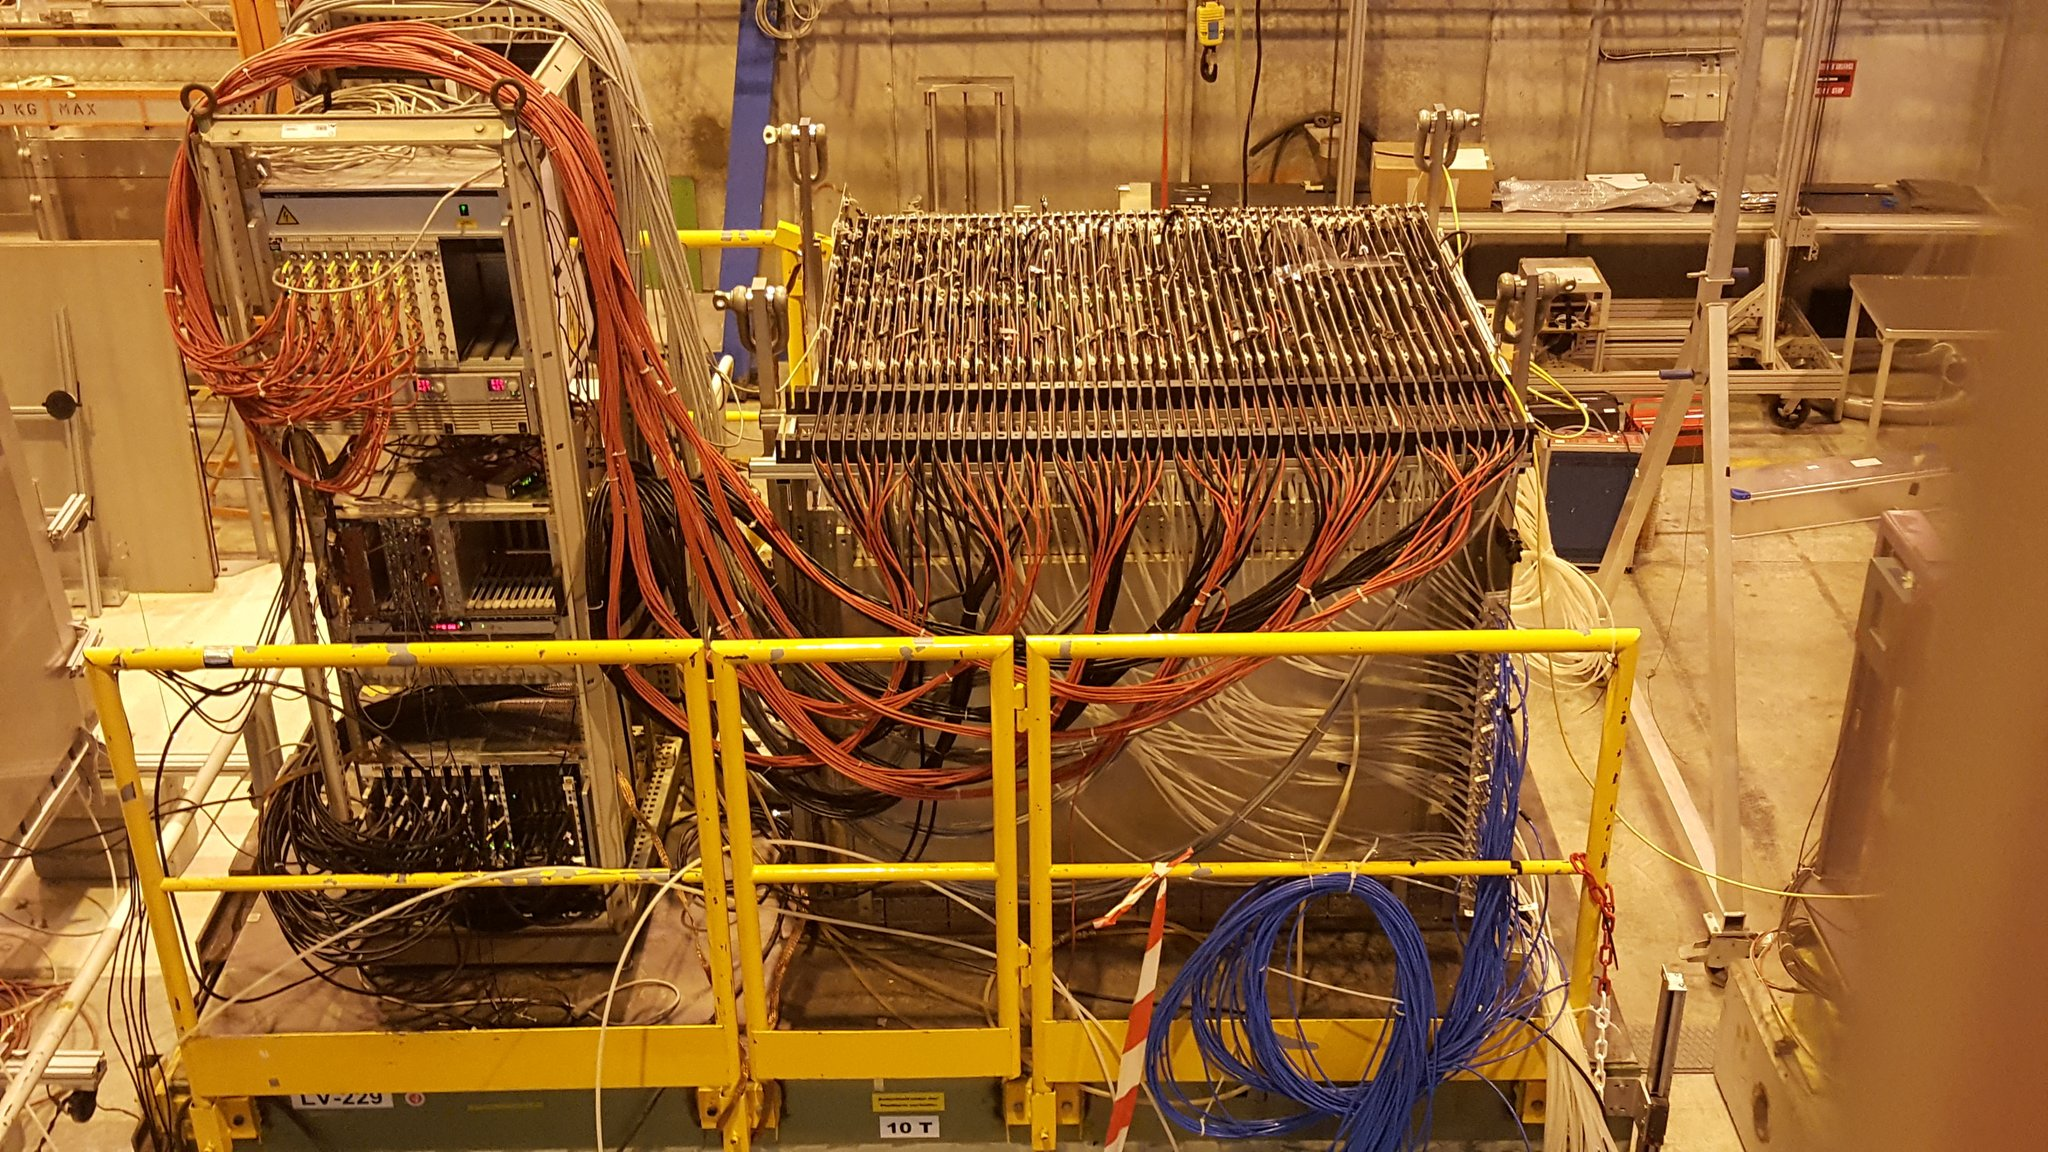
\includegraphics[width=0.8\linewidth]{Fig/sdhcal_prototype.jpeg}
    \caption{Vue du prototype SDHCAL instrumenté lors d'une campagne de test faisceau.}
    \label{fig:sdhcal_real}
\end{figure}

\section{Principe de détection dans les GRPC}

Lorsqu'une particule chargée traverse une GRPC, elle ionise le gaz contenu dans l'entrefer. Les électrons primaires produits sont accélérés par le champ électrique appliqué entre les plaques de verre, déclenchant une avalanche électronique.

Le signal induit est collecté sur les pads de lecture situés à proximité de l'anode. La charge mesurée dépend notamment du nombre d'ionisations initiales, de la position de passage de la particule, des conditions de champ électrique, de la composition du gaz et des fluctuations propres au processus d'avalanche.

Le mélange gazeux et les conditions de fonctionnement sont choisis afin d'assurer une avalanche stable, une efficacité élevée et une limitation des décharges de type streamer.

\section{Lecture semi-digitale à trois seuils}

L'originalité du SDHCAL réside dans sa lecture semi-digitale codée sur deux bits. Trois seuils de charge sont appliqués à chaque canal :

\begin{equation}
T_1 < T_2 < T_3.
\end{equation}

Chaque hit est classé selon le plus haut seuil franchi. Cette information permet de distinguer grossièrement les dépôts isolés, les régions de densité intermédiaire et les zones très denses de la gerbe.

Une lecture purement digitale fournirait uniquement une information de présence ou d'absence de hit, ce qui entraînerait une saturation dans les régions centrales des gerbes. À l'inverse, la lecture semi-digitale conserve une sensibilité à la densité locale tout en maintenant une électronique plus simple qu'une lecture analogique complète.

Les observables directement accessibles sont notamment :

\begin{itemize}
    \item le nombre total de hits ;
    \item les compteurs par seuil \(N_1\), \(N_2\), \(N_3\) ;
    \item les fractions relatives entre seuils ;
    \item les distributions spatiales des hits ;
    \item les densités locales de dépôt.
\end{itemize}

Ces informations constituent la base des méthodes de reconstruction d'énergie et d'identification hadronique étudiées dans ce mémoire.

\section{Électronique de lecture et acquisition}

L'électronique de lecture est intégrée au plus près des chambres grâce aux ASICs \textsc{HARDROC}, conçus pour les détecteurs gazeux hautement segmentés. Chaque ASIC gère plusieurs dizaines de canaux et dispose d'une mémoire locale permettant de stocker les informations avant la lecture.

Cette architecture embarquée réduit le câblage externe et rend possible l'instrumentation d'un très grand nombre de canaux. Le système peut fonctionner en mode déclenché ou en mode sans déclenchement, selon les conditions expérimentales.

Une stratégie de \emph{power pulsing} peut également être utilisée afin de réduire la consommation électrique pendant les périodes sans faisceau, un point important pour les futurs collisionneurs linéaires.

\section{Simulation et digitalisation}

L'étude présentée dans ce mémoire repose sur une chaîne de simulation basée sur l'environnement iLCSoft, utilisant Geant4 pour la propagation des particules dans le détecteur. La simulation fournit les dépôts d'énergie élémentaires dans les couches actives.

Une étape de digitalisation transforme ensuite ces dépôts physiques en hits comparables à ceux produits par l'électronique réelle. Cette étape inclut notamment :

\begin{enumerate}
    \item la sélection temporelle des dépôts ;
    \item l'application d'une efficacité de détection ;
    \item la génération d'une charge induite fluctuante ;
    \item la diffusion transverse vers les pads voisins ;
    \item l'application des trois seuils semi-digitaux ;
    \item la production des hits reconstruits.
\end{enumerate}

La sortie finale contient, pour chaque hit, ses coordonnées discrètes \((I,J,K)\), le seuil franchi, un horodatage et l'identifiant de l'événement. Ces données sont ensuite converties en formats d'analyse, notamment \texttt{ROOT} et \texttt{CSV}, pour les études de PID et de reconstruction énergétique.

\section{Validation expérimentale}

La simulation du SDHCAL doit reproduire les principales observables mesurées lors des campagnes de tests faisceau. Le prototype a notamment été étudié au CERN avec des faisceaux de muons, d'électrons et de hadrons sur une large gamme d'énergies.

La comparaison entre données et simulation porte sur plusieurs grandeurs :

\begin{itemize}
    \item le nombre total de hits par événement ;
    \item les distributions par seuil \(N_1\), \(N_2\), \(N_3\) ;
    \item l'efficacité MIP et la multiplicité des pads ;
    \item les profils longitudinaux des gerbes ;
    \item l'extension transverse ;
    \item la position du maximum de gerbe.
\end{itemize}

Ces comparaisons permettent d'ajuster les paramètres de digitalisation, de tester différentes listes de physique hadronique de Geant4 et d'estimer les incertitudes systématiques associées à la modélisation.

\section{Reconstruction de l'énergie}

Grâce à l'information multi-seuil, l'énergie incidente peut être estimée à partir d'une combinaison pondérée des compteurs de hits :

\begin{equation}
E_{\mathrm{reco}}
=
a(N_{\mathrm{tot}})N_1
+
b(N_{\mathrm{tot}})N_2
+
c(N_{\mathrm{tot}})N_3,
\end{equation}

où \(N_{\mathrm{tot}} = N_1 + N_2 + N_3\), et où les coefficients \(a\), \(b\) et \(c\) dépendent du nombre total de hits. Ils sont ajustés à partir d'échantillons de calibration.

Cette méthode exploite le fait que les seuils élevés sont corrélés aux régions de forte densité énergétique. Dans ce travail, elle sert de référence paramétrique et est comparée à des approches de régression par apprentissage automatique.

\section{Atouts et limites du concept}

Le SDHCAL présente plusieurs atouts importants :

\begin{itemize}
    \item une excellente granularité spatiale ;
    \item une imagerie détaillée des gerbes ;
    \item une lecture compacte et robuste ;
    \item des observables riches pour le PID et la reconstruction d'énergie ;
    \item une compatibilité avec les approches de type Particle Flow.
\end{itemize}

Ses principales limites sont liées à la dépendance des chambres gazeuses aux conditions opératoires, à la complexité du très grand nombre de canaux, à la nécessité d'une calibration précise et à la profondeur finie du prototype pour les plus hautes énergies.

\section{Conclusion}

Le SDHCAL représente une approche moderne de la calorimétrie hadronique, fondée sur l'exploitation de la topologie des gerbes plutôt que sur une simple mesure intégrée de l'énergie.

Sa granularité fine et sa lecture semi-digitale en font un détecteur particulièrement adapté aux études d'identification hadronique et de reconstruction d'énergie. Dans ce mémoire, il constitue le support expérimental et numérique des méthodes d'analyse développées dans les chapitres suivants.